\documentclass[12pt,a4paper]{article}

% --- Encoding and Fonts ---
\usepackage[utf8]{inputenc}   % UTF-8 encoding
\usepackage[T1]{fontenc}      % Better font encoding
\usepackage{lmodern}          % Latin Modern font

% --- Page Layout ---
\usepackage[a4paper,margin=1in]{geometry} % Page margins
\usepackage{setspace}         % Line spacing
\onehalfspacing               % 1.5 line spacing for drafting

% --- Math Support ---
\usepackage{amsmath, amssymb, amsthm} % AMS math packages
\usepackage{mathtools}                % Extra math tools
\usepackage{bm}                       % Bold math symbols
\usepackage{siunitx}                  % SI units

% --- Graphics & Figures ---
\usepackage{graphicx}         % Include images
\usepackage{caption}          % Better captions
\usepackage{subcaption}       % Subfigures
\usepackage{float}            % Improved float control

% --- Hyperlinks ---
\usepackage{xcolor}           % Colors for links
\usepackage[
    colorlinks=true,
    linkcolor=blue,
    citecolor=teal,
    urlcolor=magenta
]{hyperref}

% --- Misc Utilities ---
\usepackage{microtype}        % Better typography
\usepackage{enumitem}         % Custom lists
\usepackage{booktabs}         % Better tables
\usepackage{csquotes}         % Quotation support

\usepackage{listings}
\lstdefinelanguage{rust}{
  keywords={
    as, async, await, break, const, continue, crate, dyn, else, enum, extern, false, fn, for, if, impl, in, let, loop, match, mod, move, mut, pub, ref, return, self, Self, static, struct, super, trait, true, type, unsafe, use, where, while,
    bool, char, f32, f64, i16, i32, i64, i8, isize, usize, str, String, Option, Result, Box, Vec,
    assert, assert_eq, println, print,
    default,
  },
  sensitive=true, % Case-sensitive
  morecomment=[l]//, % Line comments
  morecomment=[s]{/*}{*/}, % Block comments
  morestring=[d]\" % Double quoted strings
}
\lstset{
  language=rust, % Set the default language to Rust
  basicstyle=\ttfamily\small, % Font style for code (typewriter, small)
  keywordstyle=\color{blue}, % Style for keywords
  commentstyle=\color{green!50!black}, % Style for comments
  stringstyle=\color{red}, % Style for strings
  identifierstyle=\color{black}, % Style for identifiers (variables, functions)
  numbers=left, % Display line numbers on the left
  numberstyle=\tiny\color{gray}, % Style for line numbers
  stepnumber=1, % Increment line numbers by 1
  numbersep=5pt, % Space between line numbers and code
  breaklines=true, % Automatically break long lines
  frame=single, % Draw a frame around the code block
  backgroundcolor=\color{gray!10}, % Light gray background
  showspaces=false, % Don't show spaces
  showtabs=false, % Don't show tabs
  tabsize=2, % How many spaces a tab is equal to
  caption={Rust Code Snippet}, % Default caption
  label={lst:rust_example} % Default label for cross-referencing
}

% --- Title Info ---
\title{Vicsek Model Simulation on Sphere}
\author{Alireza Same}
\date{\today}

\begin{document}

\maketitle

\begin{abstract}
This project introduces a high-performance simulation of the Vicsek model on a spherical manifold, designed to investigate the statistical physics of collective motion in a topologically closed environment. By constraining self-propelled particles to a spherical surface, the simulation eliminates boundary effects inherent in Euclidean models, offering a more realistic framework for studying long-range order and emergent phenomena. The implementation utilizes 3D Cartesian vectors for robust physics calculations, including geodesic motion for particle updates and parallel transport for accurate velocity comparisons, thereby avoiding singularities and ensuring geometrically correct dynamics. The framework supports configurable noise models, enabling systematic studies of the order-disorder phase transition, cluster formation, and non-equilibrium dynamics. This ensemble-based approach provides a powerful tool for large-scale investigations into the complex collective behaviors of active matter on curved surfaces, contributing to a deeper understanding of emergent phenomena in biological and physical systems\end{abstract}

\section{Spherical Manifold}
In this model, each "bird" is represented by its position and orientation on a sphere of radius \(R\). The position of a particle is defined by a point on the spherical surface, while its velocity vector is always tangent to the sphere at that specific point, maintaining a constant speed \(s\). Consequently, the state of each particle can be fully described by a compact set of three parameters: \((\theta, \phi, \alpha)\). Here, \((\theta, \phi)\) denote the standard spherical coordinates defining the particle's location on the sphere's surface. The third parameter, \(\alpha\), specifies the direction of the velocity vector within the local tangent plane at the particle's position. This angle \(\alpha\) is measured relative to the local \(\hat{e}_\theta\) (tangential) basis vector. For a clearer visualization, see Figure \ref{fig:particle_representation}.
\begin{figure}[H]
    \centering
    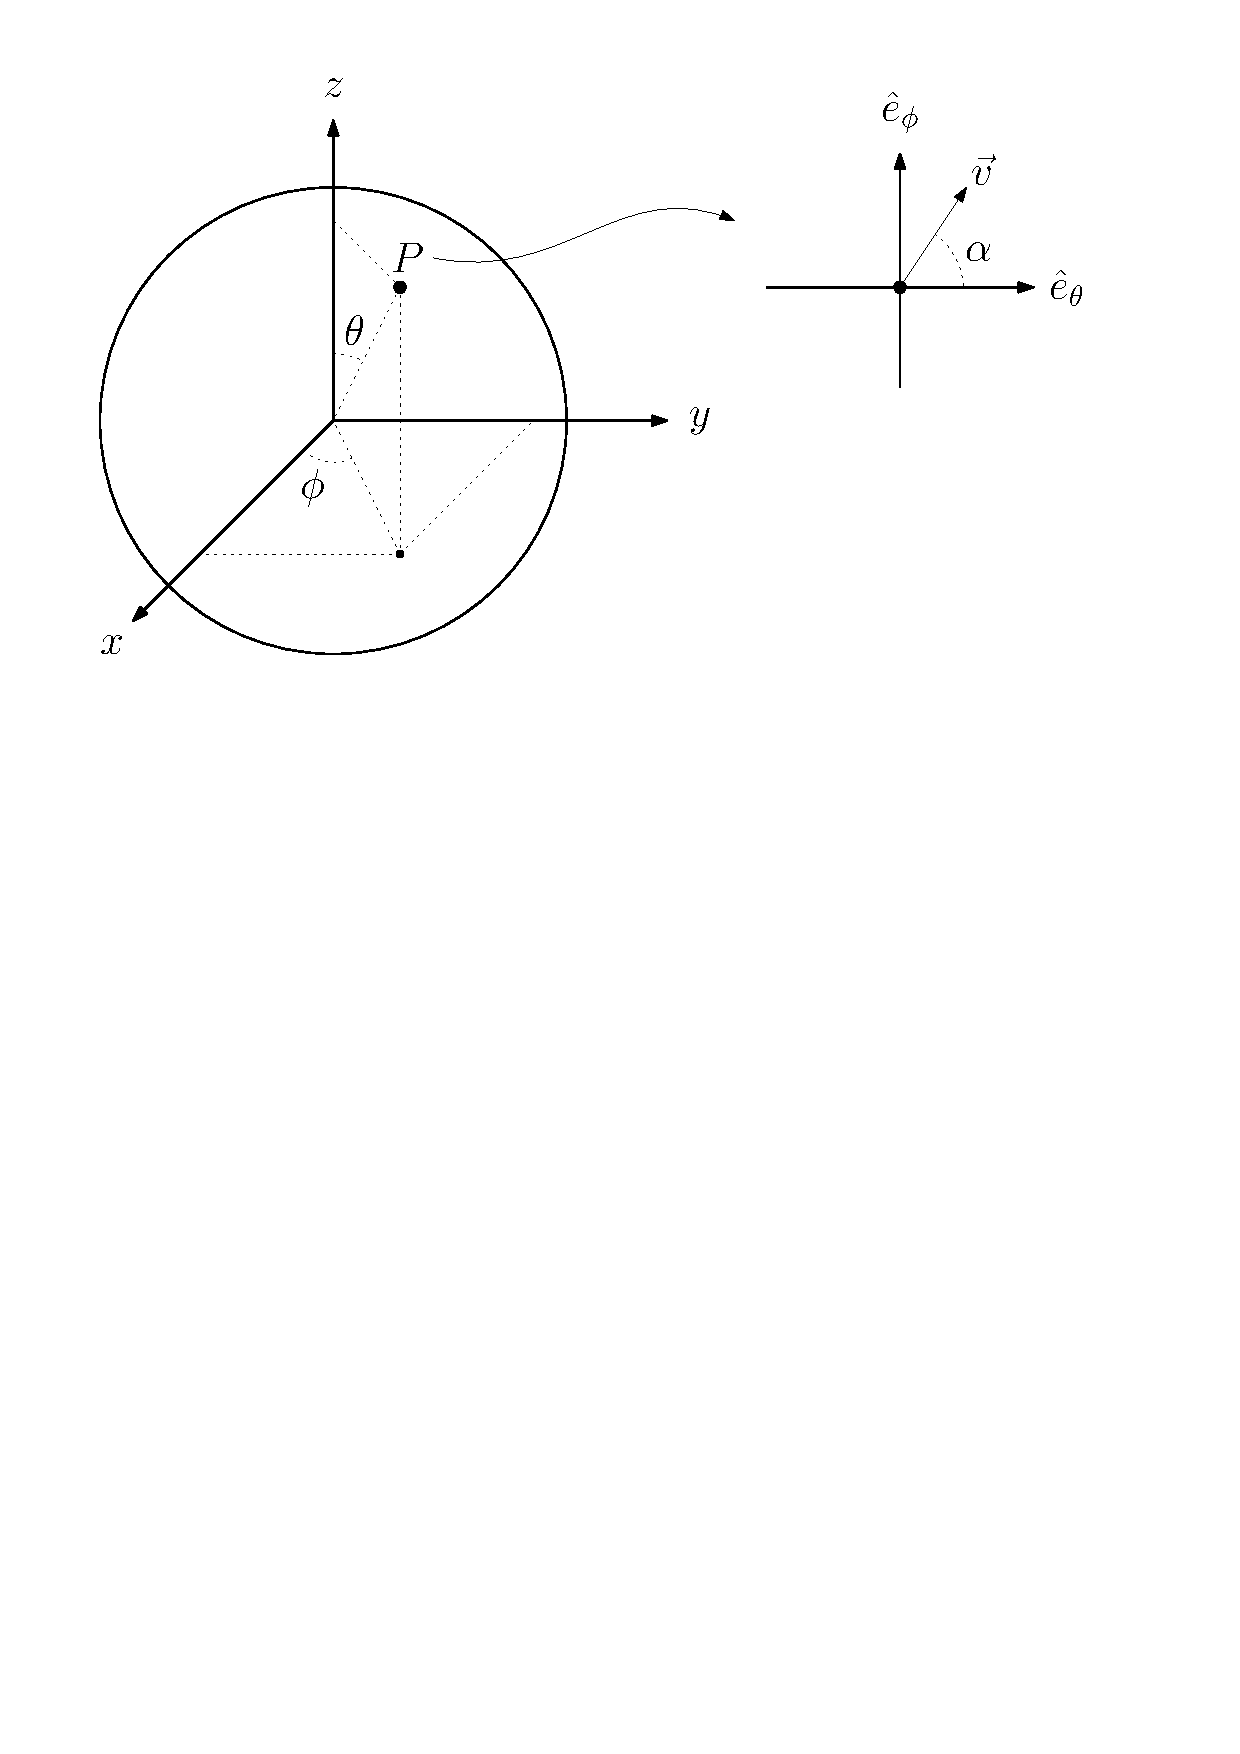
\includegraphics[width=0.6\linewidth]{./Figures/particle.pdf}
    \caption{Representation of a particle on the spherical manifold.}
    \label{fig:particle_representation}
\end{figure}

To convert the spherical coordinates \(\theta, \phi, \alpha\) to 3D Cartesian coordinates, we use the following transformations:
The Cartesian coordinates \((x, y, z)\) of a particle located at \((\theta, \phi)\) on the sphere of radius \(R\) are given by:
\begin{equation}
    \label{eq-spherical_to_cartesian}
\left\{
\begin{array}{l}
x = R \sin\theta \cos\phi \\
y = R \sin\theta \sin\phi \\
z = R \cos\theta
\end{array}
\right. , \qquad
\left\{
\begin{array}{l}
\hat{e}_r = \sin\theta \cos\phi \, \hat{i} + \sin\theta \sin\phi \, \hat{j} + \cos\theta \, \hat{k} \\
\hat{e}_\theta = \cos\theta \cos\phi \, \hat{i} + \cos\theta \sin\phi \, \hat{j} - \sin\theta \, \hat{k} \\
\hat{e}_\phi = -\sin\phi \, \hat{i} + \cos\phi \, \hat{j}
\end{array}
\right.
\end{equation}
The velocity vector \(\vec{v}\) can be expressed as follows:
\begin{equation}
    \label{eq-velocity_vector}
    \vec{v} = s \left( \cos\alpha \, \hat{e}_\theta + \sin\alpha \, \hat{e}_\phi \right)
\end{equation}
\subsection{Great-circle Distance}
In this simulation, determining the distance between two birds is crucial. We employ the great-circle distance, representing the shortest path along the Earth's surface. While typically associated with spherical coordinates, calculating this distance is simplified using Cartesian coordinates. The angle between two points on the sphere can be derived from the dot product of their position vectors. The great-circle distance \(d_{GC}\) between two points on the sphere is then given by:
\begin{equation}
    \label{eq-great_circle_distance}
    d_{GC}\left(P_1, P_2\right) = R \cdot \arccos\left( \frac{\vec{r}_1 \cdot \vec{r}_2}{R^2} \right)
\end{equation}
In our simulation, we acknowledge two singular scenarios for inter-bird distance. The first, a zero-distance case (\(d_{GC} = 0\)), signifies a collision. The second, the antipodal case (\(d_{GC} = \pi R\)), represents birds on diametrically opposite sides of the sphere, precluding visual contact. Both singularities will be excluded from the simulation. Therefore, the distance between any two birds will always satisfy \(0 < d_{GC} < \pi R\). It is important to note that a more appropriate maximal distance for certain applications, such as visibility calculations, might be \(d_{GC} = \frac{\pi}{2} R\), which significantly alters the scope of potential interactions.

\subsection{Parallel Transport}
To determine the average direction of neighboring birds, it is necessary to parallel transport their respective velocities to the base bird's position before averaging. This procedure ensures the meaningfulness of the resulting average, see Figure \ref{fig:parallel_transport}.
\begin{figure}[H]
    \centering
    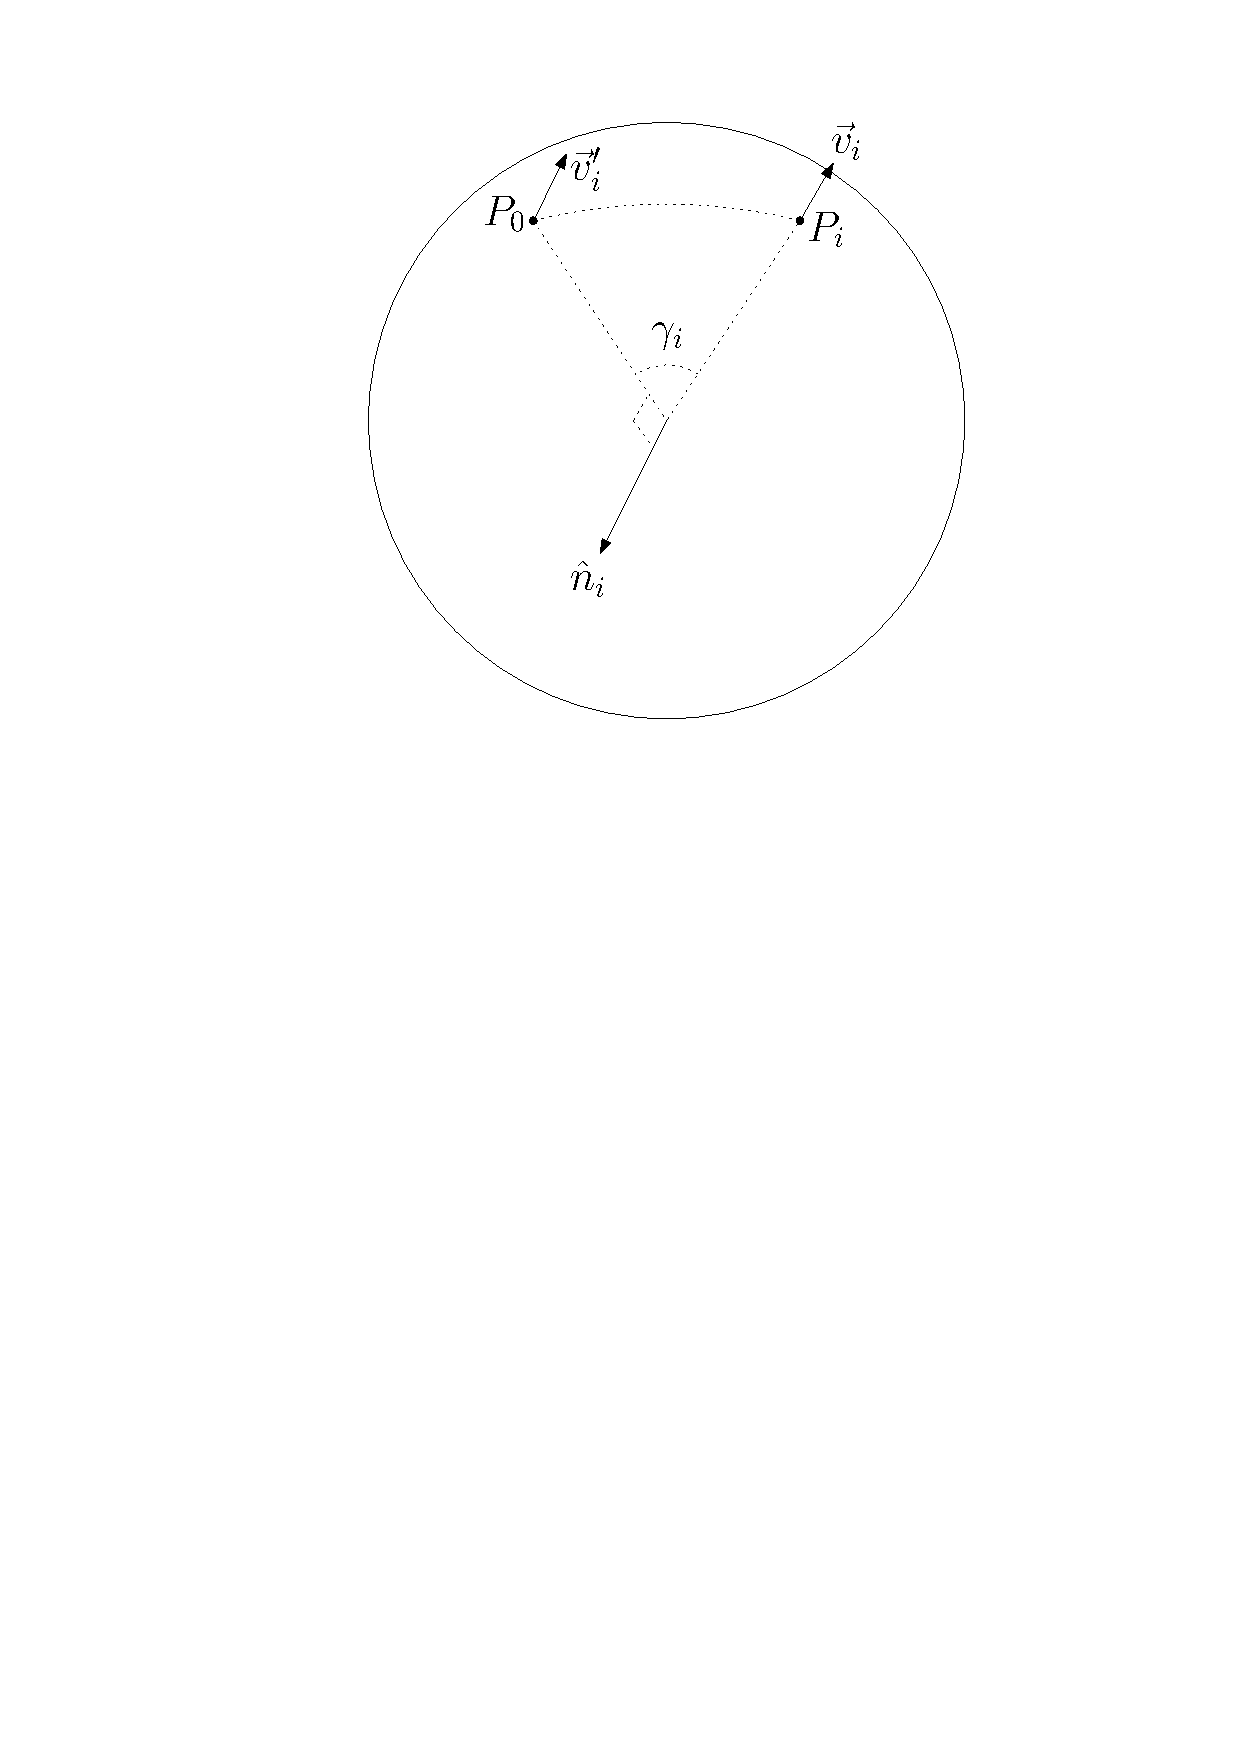
\includegraphics[width=0.3\linewidth]{Figures/parallel}
    \caption{Parallel transport of velocities}
    \label{fig:parallel_transport}
\end{figure}

Let \(P_0\) represent the base bird, and \(P_1, P_2, \ldots, P_n\) denote the \(n\) birds within its visual range. The parallel transport of the velocity vector \(\vec{v}_i\) of bird \(P_i\) to the base bird \(P_0\) is accomplished via a rotation about the appropriate axis. This rotation will be calculated using Rodrigues' rotation formula, as given by Equation (\ref{eq:rodrigues}).
\begin{align}
& \hat{n}_i = \frac{\vec{r}_i \times \vec{r}_0}{\|\vec{r}_i \times \vec{r}_0\|}, \quad \gamma_i = \arccos\left( \frac{\vec{r}_i \cdot \vec{r}_0}{R^2}\right) \\
\label{eq:rodrigues}
& \vec{v}_{i}^\prime = \vec{v}_i \cos\gamma_i + (\hat{n}_i \times \vec{v}_i) \sin\gamma_i + \hat{n}_i (\hat{n}_i \cdot \vec{v}_i) (1 - \cos\gamma_i)
\end{align}
As evident, the parallel transport operation encounters a singularity when dealing with antipodal points. Consequently, such cases are excluded from consideration. Following the parallel transport of all neighboring birds' velocities, these vectors are averaged to yield a new resultant velocity vector direction. It is important to note that this resultant vector may, in certain instances, be a zero vector. In such an eventuality, the current velocity vector of the base bird will be retained without modification. Subsequently, the derived velocity vector is normalized to maintain a constant speed \(s\). We will denote this by \(\vec{v}_{\text{ave}}\). Finally, the simulation's inherent noise component is incorporated into this normalized velocity vector.
\subsection{Noise Addition (Rotation)}
Upon determining the new direction, a small random rotation is applied. This rotation is performed within the tangent space at the current point, thereby preserving the tangency of the velocity vector. The magnitude of this rotational angle is sampled from a pre-defined distribution, which will be elaborated upon subsequently. Utilizing Rodrigues' rotation formula once more for this operation, we obtain:
\[
\vec{v}_{\text{transport}} = \vec{v}_{\text{ave}} \cos\alpha_n + (\hat{r}_0 \times \vec{v}_{\text{ave}}) \sin\alpha_n + \hat{r}_0 (\hat{r}_0 \cdot \vec{v}_{\text{ave}}) (1 - \cos\alpha_n)
\]

\subsection{Time step}

With the new velocity vector established, the bird's position and velocity are updated in two stages. First, the bird's position is advanced along a geodesic according to the new velocity vector, using a time step \(dt\). Subsequently, this new velocity vector is parallel transported to the updated position, similar to previous operations. This yields the bird's new position and velocity vector, which serve as the initial conditions for the subsequent simulation step. This inherent Markovian property, where the current state depends solely on the previous state, offers significant computational advantages. 

We know that velocity is perpendicular to position vector (tangency) this will simplify the geodesic equation to:
\begin{align}
\label{eq:geodesic}
& \vec{r}(t+dt) =  \cos\left(\frac{\|\vec{v}_{\text{transport}}\| dt}{R}\right) \vec{r}(t)+ \frac{R}{s} \sin\left(\frac{\|\vec{v}_{\text{transport}}\| dt}{R}\right) \vec{v}_{\text{transport}} \\
& \vec{v}(t+dt) =  \cos\left(\frac{\|\vec{v}_{\text{transport}}\| dt}{R}\right) \vec{v}_{\text{transport}}- \frac{s}{R} \sin\left(\frac{\|\vec{v}_{\text{transport}}\| dt}{R}\right) \vec{r}(t)
\end{align}

Two considerations are paramount during time-stepping. Firstly, to mitigate floating-point errors, the angular displacement, \(s \cdot dt\), must remain sufficiently small; specifically, it should not exceed \(\frac{\pi}{2} R\), as larger values would constitute an excessive jump. Secondly, it is imperative to manually verify and normalize the magnitudes of both the position and velocity vectors. This normalization procedure will effectively mitigate the accumulation of floating-point errors.

\section{Random Variables}
The simulation necessitates the generation of random values for both ensemble initialization and noise injection. This section will detail the methodologies employed for random number generation, including the specific probability distributions utilized.

\subsection{Ensemble generation}
To establish the initial conditions for our simulation, we must generate an ensemble of birds with randomly distributed positions. Utilizing spherical coordinates simplifies this process. For truly random sets, we employ uniform distributions for angle generation. The azimuthal angle, \(\phi\), and the angle for the initial velocity direction, \(\alpha\), are directly sampled uniformly from \(0\) to \(2\pi\). However, generating the polar angle, \(\theta\), requires a more nuanced approach. Simply sampling \(\theta\) uniformly from \(0\) to \(\pi\) would result in an disproportionate concentration of points near the poles. To achieve a truly uniform distribution of points across the spherical surface, we instead generate \(\cos\theta\) uniformly from \(-1\) to \(1\), and then derive \(\theta\) from this value. This method ensures an even spatial distribution of birds, avoiding artificial clustering at the poles.
\[
\left\{
\begin{array}{l}
    \theta = \arccos(U[-1, 1]) \\
\phi \sim U[0, 2\pi] \\
\alpha \sim U[0, 2\pi]

\end{array}
\right.
\]

For ensemble generation, we sample these three angles. A critical step involves verifying that no pre-existing bird is in close proximity to the newly generated position, thereby preventing unwanted initial collisions. Once \(N\) birds have been successfully created, this set constitutes a single ensemble, which is then saved. This process is repeated to generate a total of \(M\) ensembles, facilitating subsequent ensemble averaging.

\subsection{Noise Generation}
To introduce noise, we apply a rotational angle, \(\alpha_n\), ranging from \(-\pi\) to \(\pi\), where a value of zero signifies no rotation. This angle is sampled from a normal distribution centered at zero with a variance of \(\eta^2\), where \(\eta\) represents the noise strength parameter, ranging from zero to infinity. As \(\eta\) increases (approaching \(4\pi\)), the distribution of \(\alpha_n\) effectively becomes uniform, leading to complete randomness. Conversely, a value of \(\eta = 0\) introduces no randomness. There exists a critical value of \(\eta\) that corresponds to a phase transition within the system.
\[
\alpha_n \sim \mathcal{N}(0, \eta^2), \quad 0 \le \eta < 4\pi
\]
\section{Parameter Sensitivity Analysis}
The primary objective of this simulation is to identify phase changes within the system. Given our ensemble-based approach, a parameter sensitivity analysis is essential. For each simulation run, the following parameters will be examined individually:
\begin{itemize}
    \item \textbf{Radius ($R$)}: 
    This parameter holds no true influence on the simulation's intrinsic behavior. Its selection is primarily to mitigate numerical issues. Beyond this, the radius lacks significance, as it does not even incorporate scaling. Its sole effect is to impart a dimension to the neighbor distance parameter, rendering it largely irrelevant to the core dynamics.
    \item \textbf{Speed ($s$)}: 
    Similar to the radius, the speed parameter is also largely irrelevant. Its primary function is to establish the system's time scale in conjunction with the radius. As previously discussed, the time step must be sufficiently small to maintain logical consistency; thus, speed is a free parameter that imposes a bound on \(dt\). Beyond this, it holds no further significance in the simulation.
    \item \textbf{Neighbor Distance ($d$)}: 
    This parameter holds significant importance, though it functions more as a classifying variable than a continuous one for trend analysis. For instance, a value of \(\pi R/2 \) would correspond to a mean-field approximation of the model. Consequently, we only require approximately four distinct values of this parameter to discern its impact on the system's behavior.
    \item \textbf{Noise Strength ($\eta$)}: 
    This stands as the most crucial parameter in our simulation, as we aim to observe its continuous impact on phase transitions. We contend that noise strength is the primary catalyst for these transitions within the system. By systematically varying \(\eta\), we can observe the system's progression from ordered to disordered states, thereby revealing the critical noise level at which these phase changes manifest. Our simulation specifically targets the identification of the numerous first-order phase transitions expected in this system.
    \item \textbf{Number of Birds ($N$)}: 
    To investigate finite-size scaling effects, we must vary the number of birds in the system. Similar to the parameter \(d\), changes in this parameter are expected to reveal only minor trends. Given that this system does not exhibit continuous phase transitions, we do not anticipate observing significant finite-size scaling behavior around any noise parameter, as critical exponents are absent.
    \item \textbf{Number of Ensembles ($M$)}: 
    This parameter is crucial for ensuring statistical significance in our results. By increasing the number of ensembles, we can obtain a more reliable estimate of the average behavior of the system. However, it is important to note that beyond a certain point, increasing \(M\) yields diminishing returns in terms of improved accuracy.
    \item \textbf{Time Step ($dt$)}: 
    The time step is a critical parameter that must be chosen carefully to ensure the stability and accuracy of the simulation. A small \(dt\) is necessary to avoid numerical instabilities, especially when dealing with high-speed particles or large-radius spheres. However, excessively small time steps can lead to increased computational costs without significant benefits. Therefore, it is essential to find an optimal balance for \(dt\) that maintains the integrity of the simulation while minimizing computational overhead.
\end{itemize}

\section{Implementation Details}
The simulation is implemented in the Rust programming language. The library's functionality is organized into the following submodules:
\begin{itemize}
    \item Core Physics: \begin{itemize}
        \item bird: Defines the fundamental particle representation and their associated physics.
        \item vector: Provides optimized 3D vector mathematics crucial for spherical geometry.
    \end{itemize}
    \item Simulation Engine: \begin{itemize}
        \item simulation: Houses the high-performance, parallelized simulation loop and state management.
        \item ensemble: Facilitates the generation of initial conditions, particularly for uniform particle distribution on the sphere.
    \end{itemize}
    \item Utilities and Analysis: \begin{itemize}
        \item analysis: Implements metrics for collective behavior, such as order parameters and cluster analysis.
        \item io: Manages data persistence and serialization.
        \item cli: Defines the command-line interface for direct execution.
    \end{itemize}
\end{itemize}
\subsection{Vector Module}
The \texttt{Vec3} structure is designed to represent a vector in a 3D Cartesian coordinate system.
\begin{lstlisting}[language=rust, caption={\texttt{Vec3} struct}, label={lst:rust_main}]
#[derive(Clone, Copy, serde::Serialize, serde::Deserialize)]
pub struct Vec3 {
    pub x: f64,
    pub y: f64,
    pub z: f64,
}
\end{lstlisting}

The \texttt{Vec3} structure provides a rich set of methods for vector manipulation, creation, and mathematical operations. These methods are categorized below for clarity.

\subsubsection{Constructors and Static Methods}
\begin{itemize}
    \item \textbf{\texttt{new(x: f64, y: f64, z: f64)}}
    
    Creates a new 3D vector with the specified $x$, $y$, and $z$ components. This is the primary way to instantiate a \texttt{Vec3}.

    \item \textbf{\texttt{zero()}}

    Returns a zero vector (\(0, 0, 0\)). Useful as an origin point or additive identity.

    \item \textbf{\texttt{x\_hat()}}

    Returns the unit vector along the positive X-axis (\(1, 0, 0\)).

    \item \textbf{\texttt{y\_hat()}}

    Returns the unit vector along the positive Y-axis (\(0, 1, 0\)).

    \item \textbf{\texttt{z\_hat()}}

    Returns the unit vector along the positive Z-axis (\(0, 0, 1\)).
\end{itemize}

\subsubsection{Magnitude and Normalization Methods}
\begin{itemize}
    \item \textbf{\texttt{norm\_squared() : f64}}
    
    Calculates the squared magnitude (\(x^2 + y^2 + z^2\)) of the vector. More efficient than \texttt{norm()} as it avoids a square root.

    \item \textbf{\texttt{norm() : f64}}

    Calculates the magnitude (Euclidean length) of the vector (\(\sqrt{x^2 + y^2 + z^2}\)).

    \item \textbf{\texttt{normalize() : Self}}
    
    Returns a unit vector (\text{magnitude} = 1) in the same direction. Returns the zero vector if the original vector has zero or near-zero magnitude.
\end{itemize}

\subsubsection{Vector Operations}
\begin{itemize}
    \item \textbf{\texttt{dot(\&self, other: \&Self) : f64}}

    Calculates the dot product (scalar product) with another vector. Measures how much two vectors point in the same direction.

    \item \textbf{\texttt{cross(\&self, other: \&Self) : Self}}
    
    Calculates the cross product with another vector. Produces a vector perpendicular to both input vectors, following the right-hand rule.

    \item \textbf{\texttt{angle\_between(\&self, other: \&Self) : f64}}
    
    Calculates the angle in radians between this vector and another. The result is in the range \([0, \pi]\).

    \item \textbf{\texttt{project\_onto(\&self, other: \&Self) : Self}}
    
    Projects this vector onto another vector. The result is a vector component that lies along the direction of the target vector.

    \item \textbf{\texttt{rotate\_around(\&self, axis: \&Self, angle: f64) : Option<Self>}}
    
    Rotates this vector around a specified \emph{normalized} axis by a given angle in radians. Returns \texttt{Some(Vec3)} on success, \texttt{None} if the axis is invalid (e.g., zero vector or not normalized).
\end{itemize}

\subsubsection{Utility Functions}
\begin{itemize}
    \item \textbf{\texttt{approx\_eq(\&self, other: \&Self, epsilon: f64) : bool}}
    
    Checks if this vector is approximately equal to another within a given \texttt{epsilon} tolerance for each component, due to floating-point precision.

    \item \textbf{\texttt{Add<Vec3> for Vec3}} ($\texttt{+}$)
    Overloads the addition operator (\texttt{+}) for vector-vector addition.

    \item \textbf{\texttt{Sub<Vec3> for Vec3}} ($\texttt{-}$)
    Overloads the subtraction operator (\texttt{-}) for vector-vector subtraction.

    \item \textbf{\texttt{Mul<f64> for Vec3}} ($\texttt{*}$)
    Overloads the multiplication operator (\texttt{*}) for scalar multiplication (\texttt{Vec3 * f64}).

    \item \textbf{\texttt{Mul<Vec3> for f64}} ($\texttt{*}$)
    Overloads the multiplication operator (\texttt{*}) for commutative scalar multiplication (\texttt{f64 * Vec3}).

    \item \textbf{\texttt{Div<f64> for Vec3}} ($\texttt{/}$)
    Overloads the division operator (\texttt{/}) for scalar division (\texttt{Vec3 / f64}).

    \item \textbf{\texttt{Neg for Vec3}} ($\texttt{-}$)
    Overloads the unary negation operator (\texttt{-}) to reverse the vector's direction.

    \item \textbf{\texttt{PartialEq for Vec3}} ($\texttt{==}$)
    Implements equality comparison (\texttt{==}) for \texttt{Vec3} instances. Note that due to floating-point arithmetic, \texttt{approx\_eq} is generally preferred for meaningful comparisons.
\end{itemize}







\section{Results}
Hopefully someday


\bibliographystyle{plain}
\bibliography{references} % Create a references.bib file if needed

\end{document}